\documentclass[11pt, a4paper]{article}

% --- Packages ---
\usepackage[utf8]{inputenc}
\usepackage[T1]{fontenc}
\usepackage{geometry}
\geometry{top=2.5cm, bottom=2.5cm, left=2.5cm, right=2.5cm}
\usepackage{amsmath, amssymb, amsthm}
\usepackage{graphicx}
\usepackage[dvipsnames]{xcolor}
\usepackage{parskip} % Adds space between paragraphs, removes indentation
\usepackage{hyperref}
\usepackage{tikz}
\usepackage{pgfplots}
\pgfplotsset{compat=1.18}
\usetikzlibrary{shapes, arrows, positioning, calc}
\usepackage{tcolorbox}
\tcbuselibrary{skins, breakable}

% --- Custom Environments ---

% 1. Intuition Box (Green/Teal)
\newtcolorbox{intuitionbox}[1]{
  enhanced,
  breakable,
  colback=teal!10!white,
  colframe=teal!70!black,
  title=\textbf{💡 Intuition: #1},
  fonttitle=\bfseries,
  boxrule=0.5mm,
  attach boxed title to top left={xshift=0.5cm, yshift=-2mm},
  boxed title style={colback=teal!70!black, rounded corners},
  top=1em
}

% 2. Example Box (Blue)
\newtcolorbox{examplebox}[1]{
  enhanced,
  breakable,
  colback=blue!5!white,
  colframe=blue!60!black,
  title=\textbf{🏠 Example: #1},
  fonttitle=\bfseries,
  boxrule=0.5mm,
  attach boxed title to top left={xshift=0.5cm, yshift=-2mm},
  boxed title style={colback=blue!60!black, rounded corners},
  top=1em
}

% 3. Math Deep Dive Box (Purple)
\newtcolorbox{mathbox}[1]{
  enhanced,
  breakable,
  colback=violet!5!white,
  colframe=violet!60!black,
  title=\textbf{🧮 Math Deep Dive: #1},
  fonttitle=\bfseries,
  boxrule=0.5mm,
  attach boxed title to top left={xshift=0.5cm, yshift=-2mm},
  boxed title style={colback=violet!60!black, rounded corners},
  top=1em
}

% --- Document Info ---
\title{\textbf{The Intuitive Guide to Statistical Learning}\\ \large From Basic Concepts to the Bias-Variance Tradeoff}
\author{Machine Learning Foundations}
\date{\today}

\begin{document}

\maketitle
\tableofcontents
\newpage

\section{Statistical Learning vs. Machine Learning}

Before diving into models, it is helpful to understand the landscape. Historically, \textbf{Statistical Learning} emerged from statistics with a focus on \textit{inference}—understanding the relationship between variables (e.g., "How does smoking affect life expectancy?"). \textbf{Machine Learning} emerged from computer science with a focus on \textit{prediction}—building algorithms that can predict outcomes accurately (e.g., "Is this email spam?").

Today, the distinction is blurry. We use the terms interchangeably to refer to the set of tools for modeling and understanding complex datasets.

\section{Why Do We Need a Model?}

In the real world, we often observe an output variable $Y$ (also called the \textit{response} or \textit{target}) associated with a vector of input variables $X = (X_1, X_2, \dots, X_p)$ (also called \textit{features} or \textit{predictors}). We assume there is some underlying, fixed but unknown relationship between them, which we can write as:

\begin{equation}
    Y = f(X) + \epsilon
\end{equation}

Here:
\begin{itemize}
    \item $f: \mathbb{R}^p \to \mathbb{R}$ is the true, unknown function that systematically connects inputs to outputs.
    \item $\epsilon$ is the \textbf{random error term}, independent of $X$ and with mean zero ($E[\epsilon] = 0$). It represents noise, measurement errors, or unmeasured variables that affect $Y$ but are not in $X$.
\end{itemize}

\begin{examplebox}{Predicting Housing Prices}
Imagine we want to predict the price of a house ($Y$). The inputs ($X \in \mathbb{R}^3$) might be:
\begin{itemize}
    \item $X_1$: Square footage (Continuous)
    \item $X_2$: Number of bedrooms (Discrete)
    \item $X_3$: Distance to the city center (Continuous)
\end{itemize}

The "true" relationship $f$ might be complex and non-linear: "Add \$200 for every square foot, but subtract \$10,000 for every mile from the city, interacting with the neighborhood quality." The error $\epsilon$ captures things we didn't measure, like whether the previous owner was a smoker or if the house was renovated recently.
\end{examplebox}

We estimate $f$ for two main reasons: \textbf{Prediction} and \textbf{Inference}.

\subsection{Prediction}
If we can estimate $f$ well (let's call our estimate $\hat{f}$), we can predict $Y$ for new inputs $X$:
\[ \hat{Y} = \hat{f}(X) \]
Here, we don't care exactly \textit{how} $\hat{f}$ works, as long as $\hat{Y}$ is close to $Y$. This is a "Black Box" approach common in deep learning.

\subsection{Inference}
Sometimes we want to understand the \textit{nature} of the relationship.
\begin{itemize}
    \item Which predictors ($X$) are most important?
    \item Is the relationship linear?
    \item Does increasing $X_1$ increase or decrease $Y$?
\end{itemize}
For inference, we prefer simple, interpretable models (like Linear Regression) over complex "Black Boxes."

\begin{intuitionbox}{Reducible vs. Irreducible Error}
No matter how good our model $\hat{f}$ is, we can never perfectly predict $Y$ because of the error term $\epsilon$.
\[ E[(Y - \hat{Y})^2] = \underbrace{[f(X) - \hat{f}(X)]^2}_{\text{Reducible Error}} + \underbrace{\text{Var}(\epsilon)}_{\text{Irreducible Error}} \]
\begin{itemize}
    \item \textbf{Reducible Error}: We can reduce this by choosing a better model.
    \item \textbf{Irreducible Error}: This is the noise in the universe. We cannot eliminate it.
\end{itemize}
\end{intuitionbox}

\section{How Do Models Learn?}

"Learning" basically means using a set of observed data (the \textbf{Training Data}) to calculate the best possible $\hat{f}$.

Suppose we have $n$ observations:
\[ \mathcal{T} = \{(x_1, y_1), (x_2, y_2), \dots, (x_n, y_n)\} \]
where each $x_i \in \mathbb{R}^p$ and $y_i \in \mathbb{R}$.

Our goal is to find a function $\hat{f}$ such that $Y \approx \hat{f}(X)$ for any new observation $(X, Y)$. Formally, we want to minimize a \textbf{Loss Function} $L(Y, \hat{f}(X))$, which quantifies the "cost" of a bad prediction.

\begin{mathbox}{Empirical Risk Minimization}
We cannot directly minimize the error on future data (because we don't have it yet!). Instead, we minimize the \textbf{Empirical Risk} (the average loss on our training data):
\[ \hat{f} = \underset{f \in \mathcal{H}}{\text{argmin}} \frac{1}{n} \sum_{i=1}^{n} L(y_i, f(x_i)) \]
where $\mathcal{H}$ is the hypothesis space (the set of all possible functions our model can learn).
\end{mathbox}

\section{Approaches to Estimating $f$}

Broadly speaking, most statistical learning methods fall into two categories: \textbf{Parametric} and \textbf{Non-Parametric}.

\subsection{Parametric Methods}
This approach reduces the problem of estimating $f$ to estimating a set of parameters. It involves two steps:
\begin{enumerate}
    \item \textbf{Assumption}: We assume a functional form for $f$. For example, we might assume $f$ is linear:
    \[ f(X) = \beta_0 + \beta_1 X_1 + \beta_2 X_2 + \dots + \beta_p X_p \]
    \item \textbf{Fitting}: We use the training data to fit (estimate) the coefficients $\beta_0, \beta_1, \dots, \beta_p$.
\end{enumerate}

The most common method is \textbf{Ordinary Least Squares (OLS)}. We look for the coefficients $\hat{\beta}$ that minimize the sum of squared differences between the observed values and the predicted linear values:
\[ \hat{\beta} = \underset{\beta}{\text{argmin}} \sum_{i=1}^{n} (y_i - \beta^T x_i)^2 \]
This optimization problem has a beautiful "closed-form" solution (calculated using matrix algebra) that guarantees the best linear fit.

\begin{intuitionbox}{Parametric Tradeoff}
\textbf{Pros:} Simple, easy to interpret, requires less data. \\
\textbf{Cons:} The assumption might be wrong! If the true $f$ is very wiggly and we assume a straight line, our estimate will be poor (High Bias).
\end{intuitionbox}

\subsection{Non-Parametric Methods}
Non-parametric methods do not make explicit assumptions about the functional form of $f$. Instead, they seek an estimate that is as close to the data points as possible without being too rough or wiggly.

A classic example is \textbf{K-Nearest Neighbors (KNN)}. For any given input $x_0$, KNN identifies the $K$ points in the training data that are closest to $x_0$ (represented by the set $\mathcal{N}_0$). It then estimates $f(x_0)$ as the average of the response values for these neighbors:
\[ \hat{f}(x_0) = \frac{1}{K} \sum_{x_i \in \mathcal{N}_0} y_i \]

\begin{intuitionbox}{Non-Parametric Tradeoff}
\textbf{Pros:} Can fit a wide range of shapes accurately. \\
\textbf{Cons:} Requires a LOT of data to get an accurate estimate. Can easily "overfit" (follow the noise in the data).
\end{intuitionbox}

\begin{figure}[h]
    \centering
    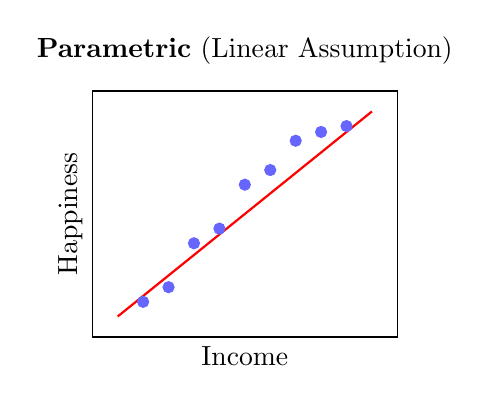
\begin{tikzpicture}
        \begin{axis}[
            width=0.45\textwidth,
            title={\textbf{Parametric} (Linear Assumption)},
            xlabel={Income}, ylabel={Happiness},
            xtick=\empty, ytick=\empty,
            domain=0:10,
            samples=20
        ]
            % Scatter points (True data is curved)
            \addplot[only marks, mark=*, blue!60] coordinates {
                (1, 2) (2, 2.5) (3, 4) (4, 4.5) (5, 6) (6, 6.5) (7, 7.5) (8, 7.8) (9, 8)
            };
            % Linear Fit
            \addplot[thick, red] coordinates {(0, 1.5) (10, 8.5)};
        \end{axis}
    \end{tikzpicture}
    \hfill
    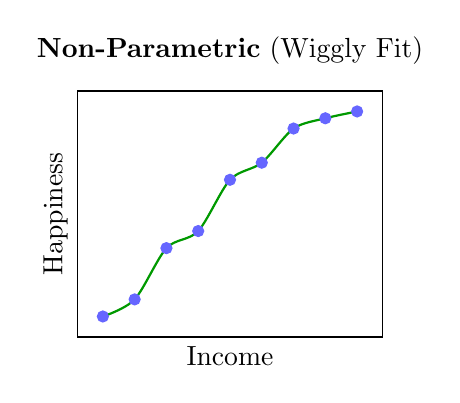
\begin{tikzpicture}
        \begin{axis}[
            width=0.45\textwidth,
            title={\textbf{Non-Parametric} (Wiggly Fit)},
            xlabel={Income}, ylabel={Happiness},
            xtick=\empty, ytick=\empty,
            domain=0:10
        ]
            % Scatter points
            \addplot[only marks, mark=*, blue!60] coordinates {
                (1, 2) (2, 2.5) (3, 4) (4, 4.5) (5, 6) (6, 6.5) (7, 7.5) (8, 7.8) (9, 8)
            };
            % Wiggly Fit (Spline-like)
            \addplot[thick, green!60!black, smooth] coordinates {
                (1, 2) (2, 2.5) (3, 4) (4, 4.5) (5, 6) (6, 6.5) (7, 7.5) (8, 7.8) (9, 8)
            };
        \end{axis}
    \end{tikzpicture}
    \caption{\textbf{Left:} A parametric model assumes a shape (line) which may miss the curvature. \textbf{Right:} A non-parametric model adapts to the data but may follow noise.}
\end{figure}

\section{Assessing Model Accuracy}

There is no "free lunch" in statistics: no one method dominates all others over all possible datasets. To choose the best model, we need to measure how well it performs.

\subsection{Training vs. Test Error}
In regression settings, the most common quality measure is the \textbf{Mean Squared Error (MSE)}. For the training data $\mathcal{T}$, the \textbf{Training MSE} is:
\[ MSE_{Tr} = \frac{1}{n} \sum_{i=1}^{n} (y_i - \hat{f}(x_i))^2 \]

However, we are interested in the accuracy of $\hat{f}$ on \textit{unseen} test data. If $(x_0, y_0)$ is a new observation drawn from the population, the \textbf{Test MSE} is:
\[ MSE_{Te} = E[(y_0 - \hat{f}(x_0))^2] \]
where the expectation averages over the randomness in the new data point.

\begin{intuitionbox}{The Student Analogy}
Imagine a student preparing for an exam.
\begin{itemize}
    \item \textbf{Training Data $\mathcal{T}$:} The textbook practice problems.
    \item \textbf{Model $\hat{f}$:} The student's knowledge (rules they learned).
    \item \textbf{Training Error:} The score on the textbook problems.
    \item \textbf{Test Data $(X_{new}, Y_{new})$:} The actual exam questions (which differ from the book).
    \item \textbf{Generalization Error:} The expected score on the exam.
\end{itemize}
A student who memorizes the answers to the practice problems (Overfitting) will have near-zero Training Error but huge Test Error!
\end{intuitionbox}

\section{The Bias-Variance Tradeoff}

This is arguably the most important concept in machine learning theory. It explains \textit{why} models fail. Before deriving it, we need to understand a key mathematical tool.

\begin{mathbox}{A Primer on Expectation ($E$)}
In probability, the \textbf{Expectation} (denoted $E[\cdot]$) is essentially a fancy word for "Average" or "Mean" in the long run.

\textbf{Example:} Rolling a Die.
If you roll a fair die, the outcome $X$ can be 1, 2, 3, 4, 5, or 6. The average of one roll is random. But if you roll it a billion times, the average value will settle at:
\[ E[X] = 3.5 \]

\textbf{In Machine Learning:}
When we talk about the "Expected Test MSE" or $E[\hat{f}(x)]$, we are imagining a "Multiverse" scenario:
\begin{itemize}
    \item \textbf{Universe A:} We collect a dataset, train a model, get a line $\hat{f}_A$.
    \item \textbf{Universe B:} We collect a \textit{slightly different} dataset (same process, different random noise), train a model, get a line $\hat{f}_B$.
    \item \textbf{Universe C, D, ...:} Repeat ad infinitum.
\end{itemize}
$E[\hat{f}(x)]$ is the \textbf{average curve} obtained across all these infinite universes.
\end{mathbox}

\subsection{Decomposing the Error: The Mathematical Proof}

Let's rigorously derive the decomposition of the Expected Test MSE at a fixed point $x_0$.
Recall that $Y = f(x_0) + \epsilon$, where $E[\epsilon] = 0$ and $\text{Var}(\epsilon) = \sigma_\epsilon^2$. We assume $\epsilon$ is independent of $\hat{f}$.

We want to find $E[(Y - \hat{f}(x_0))^2]$.

\textbf{Step 1: Add and subtract $f(x_0)$.}
\begin{align*}
    E[(Y - \hat{f}(x_0))^2] &= E[(f(x_0) + \epsilon - \hat{f}(x_0))^2] \\
                            &= E[((f(x_0) - \hat{f}(x_0)) + \epsilon)^2]
\end{align*}

\textbf{Step 2: Expand the square $(A+B)^2 = A^2 + B^2 + 2AB$.}
\[ = E[(f(x_0) - \hat{f}(x_0))^2 + \epsilon^2 + 2(f(x_0) - \hat{f}(x_0))\epsilon] \]

\textbf{Step 3: Distribute the Expectation (Linearity of $E$).}
\[ = E[(f(x_0) - \hat{f}(x_0))^2] + E[\epsilon^2] + 2E[(f(x_0) - \hat{f}(x_0))\epsilon] \]

Since $\epsilon$ is independent of $\hat{f}$, $E[(f - \hat{f})\epsilon] = E[f - \hat{f}] \cdot E[\epsilon]$.
Since $E[\epsilon] = 0$, this whole cross-term vanishes.
Also, $E[\epsilon^2] = \text{Var}(\epsilon) + (E[\epsilon])^2 = \sigma_\epsilon^2$.

So we are left with:
\[ = E[(f(x_0) - \hat{f}(x_0))^2] + \sigma_\epsilon^2 \]

\textbf{Step 4: Expand the remaining term.}
Now consider $E[(f(x_0) - \hat{f}(x_0))^2]$. We add and subtract $E[\hat{f}(x_0)]$ inside:
\begin{align*}
    E[(f(x_0) - E[\hat{f}(x_0)] + E[\hat{f}(x_0)] - \hat{f}(x_0))^2]
\end{align*}
Let $A = f(x_0) - E[\hat{f}(x_0)]$ (This is the Bias, a constant).
Let $B = E[\hat{f}(x_0)] - \hat{f}(x_0)$ (This is the deviation from the mean).

Expanding $(A+B)^2$ again:
\[ = \underbrace{(f(x_0) - E[\hat{f}(x_0)])^2}_{\text{Bias}^2} + \underbrace{E[(E[\hat{f}(x_0)] - \hat{f}(x_0))^2]}_{\text{Variance}} + \underbrace{2(f(x_0) - E[\hat{f}(x_0)]) E[E[\hat{f}(x_0)] - \hat{f}(x_0)]}_{\text{Zero}} \]
The cross-term is zero because $E[E[\hat{f}] - \hat{f}] = E[\hat{f}] - E[\hat{f}] = 0$.

\textbf{Final Result:}
\begin{equation}
    E[(y_0 - \hat{f}(x_0))^2] = \underbrace{[\text{Bias}(\hat{f}(x_0))]^2}_{\text{Systematic Error}} + \underbrace{\text{Var}(\hat{f}(x_0))}_{\text{Estimation Error}} + \underbrace{\text{Var}(\epsilon)}_{\text{Irreducible Error}}
\end{equation}

\subsection{The Tradeoff}
As we increase the complexity (flexibility) of a model:
\begin{itemize}
    \item \textbf{Bias decreases}: The model can fit the data better.
    \item \textbf{Variance increases}: The model starts fitting the noise.
\end{itemize}

We want to find the "Sweet Spot" where the Total Error (Bias + Variance) is minimized.

\begin{figure}[h]
    \centering
    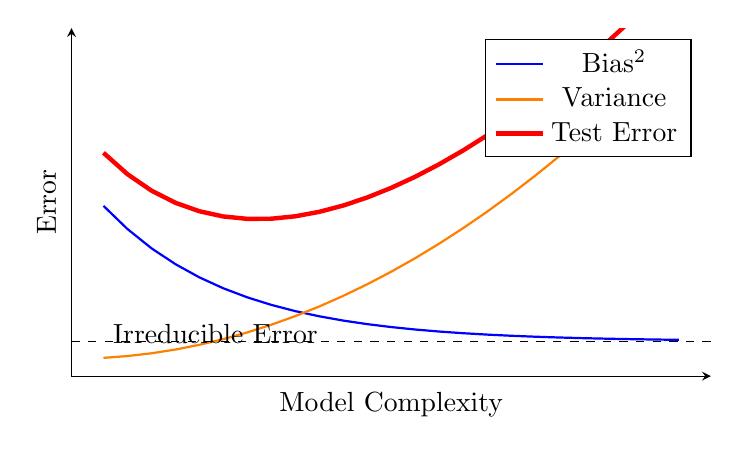
\begin{tikzpicture}
        \begin{axis}[
            width=0.8\textwidth, height=6cm,
            xlabel={Model Complexity}, ylabel={Error},
            xtick=\empty, ytick=\empty,
            xmin=0, xmax=10, ymin=0, ymax=10,
            axis lines=left,
            legend pos=north east
        ]
            % Squared Bias (Decreases)
            \addplot[blue, thick, domain=0.5:9.5] {5*exp(-0.5*x) + 1};
            \addlegendentry{Bias$^2$}

            % Variance (Increases)
            \addplot[orange, thick, domain=0.5:9.5] {0.1*x^2 + 0.5};
            \addlegendentry{Variance}

            % Test Error (U-shape)
            \addplot[red, ultra thick, domain=0.5:9.5] {5*exp(-0.5*x) + 1 + 0.1*x^2 + 0.5 + 1}; % +1 for irreducible
            \addlegendentry{Test Error}

            % Irreducible Error (Constant)
            \addplot[black, dashed, domain=0:10] {1};
            \node[right] at (axis cs: 0.5, 1.2) {Irreducible Error};

        \end{axis}
    \end{tikzpicture}
    \caption{\textbf{The Bias-Variance Tradeoff}. As complexity increases, bias drops but variance rises. The Test Error is U-shaped.}
\end{figure}

\section{Overfitting vs. Underfitting}
\begin{itemize}
    \item \textbf{Underfitting (High Bias)}: The model is too simple to capture the underlying structure of the data. Example: Using a linear model for complex housing price data.
    \item \textbf{Overfitting (High Variance)}: The model fits the training data too well, including the noise. Example: A complex polynomial that passes through every single house price point but fails on new houses.
\end{itemize}

\begin{examplebox}{Medical Diagnosis (Classification)}
Consider a model trying to predict if a patient has a disease based on Age and Blood Pressure.
\begin{itemize}
    \item \textbf{Underfitting:} The model draws a simple straight line that misses many sick patients.
    \item \textbf{Overfitting:} The model draws a crazy, wiggly curve that perfectly circles every sick patient in the training set (even the mislabeled ones). When a new patient arrives, this "wiggly" boundary makes a wild, incorrect prediction.
\end{itemize}
\end{examplebox}

\section{Estimating Test Error with Cross-Validation}

Since we often have limited data, we cannot afford to set aside a large chunk just for testing. \textbf{Cross-Validation} solves this by efficiently using the available training data to estimate the Test MSE.

\subsection{Leave-One-Out Cross-Validation (LOOCV)}
LOOCV is a special case of K-Fold where $K=n$. For every single data point $i$:
\begin{enumerate}
    \item Train the model on all data \textit{except} point $i$.
    \item Test the model on point $i$ to get $MSE_i = (y_i - \hat{f}_{-i}(x_i))^2$.
\end{enumerate}
The final estimate is the average of all $n$ MSEs.
\[ CV_{(n)} = \frac{1}{n} \sum_{i=1}^n MSE_i \]
\textbf{Bias-Variance Profile:}
\begin{itemize}
    \item \textbf{Bias (Low):} We train on $n-1$ points, which is almost as good as training on all $n$ points.
    \item \textbf{Variance (High):} We are averaging the outputs of $n$ models. However, these models are trained on almost identical datasets (they share $n-2$ points). Because the model outputs are highly correlated, their average has higher variance than averaging outputs from less correlated models.
\end{itemize}

\subsection{K-Fold Cross-Validation}
This is the gold standard. We randomly divide the data into $K$ equal-sized parts (folds) $C_1, C_2, \dots, C_K$. For each fold $k$ (from 1 to $K$):
\begin{enumerate}
    \item Treat fold $C_k$ as the Test Set.
    \item Train on the remaining $K-1$ folds.
    \item Calculate MSE on fold $k$: $MSE_k = \frac{1}{|C_k|} \sum_{i \in C_k} (y_i - \hat{f}_{-k}(x_i))^2$.
\end{enumerate}
The final estimate is the average of the $K$ MSEs:
\[ CV_{(K)} = \frac{1}{K} \sum_{k=1}^K MSE_k \]

\textbf{Bias-Variance Profile (vs LOOCV):}
\begin{itemize}
    \item \textbf{Bias (Higher):} We train on fewer points ($(K-1)/K \times n$), so the model is slightly worse.
    \item \textbf{Variance (Lower):} The overlap between training sets is smaller than in LOOCV, leading to less correlated models and a more stable estimate of the test error.
\end{itemize}
Common values for $K$ are 5 or 10, which empirically provide the best trade-off.

\begin{figure}[h]
    \centering
    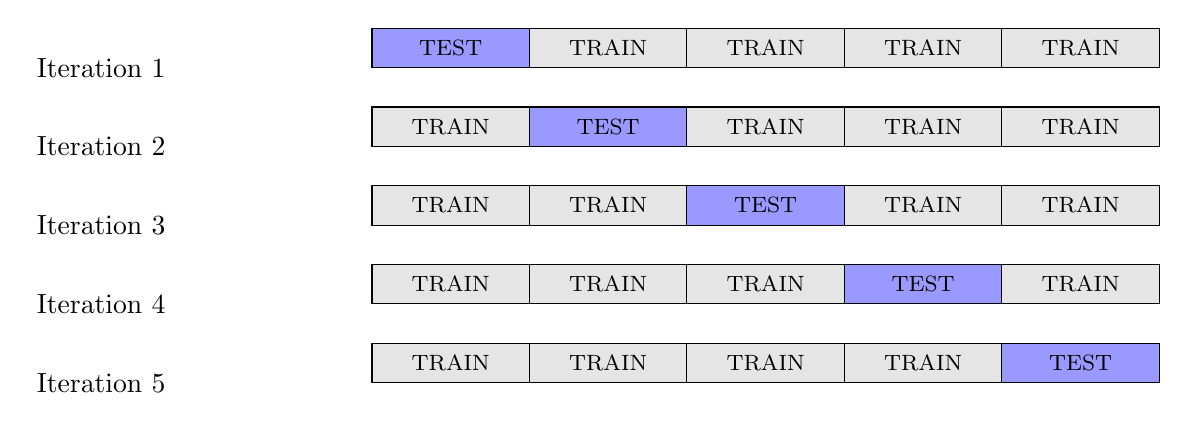
\begin{tikzpicture}
        % Define dimensions
        \def\w{2} % width of a block
        \def\h{0.5} % height of a block

        \foreach \i in {1,...,5} {
            % Draw the row label
            \node[anchor=east] at (-0.5, -\i + 1) {Iteration \i};

            % Draw the 5 blocks
            \foreach \j in {1,...,5} {
                % Set color and text based on condition
                \ifnum\i=\j
                    \def\currcolor{blue!40}
                    \def\currtext{TEST}
                \else
                    \def\currcolor{gray!20}
                    \def\currtext{TRAIN}
                \fi

                % Draw rectangle
                \draw[fill=\currcolor] (\j*\w, -\i + 1) rectangle (\j*\w + \w, -\i + 1 + \h);
                \node at (\j*\w + \w/2, -\i + 1 + \h/2) {\footnotesize \currtext};
            }
        }
    \end{tikzpicture}
    \caption{\textbf{5-Fold Cross-Validation}. In each iteration, a different part of the data is held out for testing. This ensures every data point is used for testing exactly once.}
\end{figure}

\section{Conclusion}
We have journeyed from the basic definition of statistical learning to the complex trade-offs involved in model selection.
\begin{itemize}
    \item We learned that $Y = f(X) + \epsilon$.
    \item We explored Parametric (Linear) vs. Non-Parametric (Flexible) methods.
    \item We discovered that the key to a good model is minimizing the Test Error, not the Training Error.
    \item We decomposed this error into Bias and Variance, finding that an intermediate complexity often yields the best results.
    \item Finally, we used Cross-Validation to estimate this error robustly.
\end{itemize}

\end{document}
